%%%%%%%%%%%%%%%%%%%%%%%%%%%%%%%%%%%%%%%%%%%%%%%%%%%%%%%%%%%%%%%%%%%%%%%%%%%%%%%%%%%%
%Do not alter this block of commands.  If you're proficient at LaTeX, you may include additional packages, create macros, etc. immediately below this block of commands, but make sure to NOT alter the header, margin, and comment settings here. 
\documentclass[12pt]{article}
 \usepackage[margin=1in]{geometry} 
\usepackage{amsmath,amsthm,amssymb,amsfonts, enumitem, fancyhdr, color, hyperref,comment, graphicx, environ,mathtools, bbm, tikz, setspace, cleveref,listings, dcolumn}
\usepackage{array, multirow, caption, booktabs}
\usepackage{ mathrsfs }
\usetikzlibrary{matrix,positioning}
\tikzset{bullet/.style={circle,draw=black,inner sep=8pt}}
\DeclareMathOperator*{\argmax}{arg\,max}
\DeclareMathOperator*{\argmin}{arg\,min}
\DeclareMathOperator*{\Var}{\text{Var}}
\DeclareMathOperator*{\Cov}{\text{Cov}}

\DeclarePairedDelimiter\norm{\lVert}{\rVert}%
\newtheorem{theorem}{Theorem}
\newtheorem{lemma}[theorem]{Lemma}
\DeclareMathOperator{\eps}{\varepsilon}
\doublespacing
\DeclarePairedDelimiter\abs{\lvert}{\rvert}%
\pagestyle{fancy}
\setlength{\headheight}{65pt}
\newenvironment{problem}[2][Problem]{\begin{trivlist}
\item[\hskip \labelsep {\bfseries #1}\hskip \labelsep {\bfseries #2.}]}{\end{trivlist}}
\newenvironment{sol}
    {\emph{Solution:}
    }
    {
    \qed
    }


%%%%%%%%%%%%%%%%%%%%%%%%%%%%%%%%%%%%%%%%%%%%%%%%%%%%%%%%%%%%%%%%%%%%%%%%%%%%%%%%%


\usepackage{xcolor}
 
 


%%%%%%%%%%%%%%%%%%%%%%%%%%%%%%%%%%%%%%%%%%%%%

\rhead{Asha Bharadwaj, Caitlin Dutta, John Higgins, Alexis Smith\\Econ 899 \\ 19 October, 2022} 

%%%%%%%%%%%%%%%%%%%%%%%%%%%%%%%%%%%%%%%%%%%%%


%%%%%%%%%%%%%%%%%%%%%%%%%%%%%%%%%%%%%%

\begin{document}
\begin{problem}{1}
\end{problem}
\begin{sol}
    Consider the data generating process given by  $\{x_t\}_{t=0}^T$ where $x_t = \rho_0 x_{t-1} + \eps_t$ with $\eps_t \sim N(0, \sigma^2_0)$, $\rho_0 = 0.5$, $\sigma_0 = 1$, $x_0 = 0$, and $T = 200$. The model generation process with parameter $b = (\rho, \sigma^2)$ is the following: $y_t(b) = \rho y_{t-1}(b) + e_t$, where $e_t \sim N(0,\sigma^2)$ are iid. We seek to find the asymptotic moments of the data-generating process associated with $m_3(z_t)$:
    \[m_3(z_t) = \begin{bmatrix} z_t\\(z_t - \bar{z_t})^2\\ (z_t - \bar{z})(z_{t-1} - \bar{z})\end{bmatrix}\]
    This requires us to compute the mean, variance, and first order autocorrelation. We start by computing the mean (the first component). Note that
    \[E[x_t] = E[\rho x_{t-1} +  \eps_t] = \rho E[x_{t-1}] + E[\eps_t] = \rho E[x_{t-1}]\]
    which follows from the assumption that $E[\eps_t] = 0$ $\forall t$. We also know that $x_0 = 0$. Combining this with the above, we have that $E[x_1] = \rho E[x_0] = 0$. By induction, we can see that $\forall t$, $E[x_t] = \rho E[x_{t-1}] = 0$. Thus, the mean of the process will be zero.

    We now wish to find the variance. Recognizing that $\bar{x} = 0$, we deduce the following:
    \[E[(x_t - \bar{x})^2] = E[x_t^2] = E[(\rho x_{t-1} + \eps_t)^2] = \rho^2 E[x_{t-1}^2] + 2\rho E[x_{t-1} \eps_t] + E[\eps_t^2]\]
    Furthermore, noting that $E[x_{t-1} \eps_t] = 0$ (since $\eps_t$ are iid) and $E[\eps_t^2] = \sigma^2$, we have the following:
    \[\rho^2 E[x_{t-1}^2] + 2\rho E[x_{t-1} \eps_t] + E[\eps_t^2] = \rho^2 E[x_{t-1}^2] + \sigma^2\]
    We now consider $t = 1$. From above, we have
    \[E[(x_1 - \bar{x})^2] = E[x_1^2] = \rho^2 E[x_{0}^2] + \sigma^2 = \rho^2 E[(0)^2] + \sigma^2 = \sigma^2\]
    Thus, we see that $\forall t$, $Var(x_t) = \rho^2 Var(x_{t-1}) + \sigma^2$. Starting from $\Var(x_0) = 0$ and $\Var(x_1) = \sigma^2$, it follows that 
    \begin{align*}Var(x_t) &= \rho^2 Var(x_{t-1}) + \sigma^2 \\
        &= \rho^2 (\rho^2 Var(x_{t-2}) + \sigma^2) + sigma^2\\
        &= \rho^{2t} Var(x_{0}) + \sum_{i=0}^t \sigma^2 \rho^{2i}\\
        &= \sigma^2 \sum_{i=0}^t \rho^{2i}
    \end{align*}
    Taking the limit as $t \rightarrow \infty$, we find that 
    \[\lim_{t \rightarrow \infty} Var(x_t) = \lim_{t \rightarrow \infty} \sigma^2 \sum_{i=0}^t \rho^{2i} = \frac{\sigma^2}{1 - \rho^2} \]
    Hence, the asymptotic variance is $\frac{\sigma^2}{1-\rho^2}$.

    We finally want to find the first order autocovariance. We do so below:
    \begin{align*}
        E[(x_t - \bar{x})(x_{t-1} - \bar{x})] &= E[(x_t )(x_{t-1})]\\
        &= E[(\rho x_{t-1} + \eps_t)x_{t-1}]\\
        &= \rho E[x_{t-1}^2] + E[\eps_t x_{t-1}]\\
        &= \rho \Var(x_{t-1})\\
        &= \frac{\rho \sigma^2}{1 - \rho^2}
    \end{align*}
    Putting this altogether, we get that
    \[m_3(x) = \begin{bmatrix} 0 \\\frac{\sigma^2}{1-\rho^2}\\\frac{\rho \sigma^2}{1 - \rho^2}\end{bmatrix}\]
    We can see that the second and third elements of $m_3(x_t)$ will be informative for estimating $b$. 

    Finally, we need to compute $\nabla_b g(b_0)$, where $g(b) = M_T(b) - M_{TH}(b_0)$. We find that
    \[\frac{\partial m_3(b_0)}{\partial \rho} = \begin{bmatrix} 0\\\frac{2\rho_0 \sigma_0^2}{(1-\rho_0^2)^2}\\ \frac{\sigma_0^2 (1 + \rho_0^2)}{(1 - \rho_0^2)^2}\end{bmatrix}\]
    Also,
    \[\frac{\partial m_3(b_0)}{\partial \sigma^2} = \begin{bmatrix} 0\\\frac{1}{1-\rho_0^2}\\\frac{\rho_0}{1-\rho_0^2}\end{bmatrix}\]
    Thus,
    \[\nabla_b g(b_0) = \begin{bmatrix}\frac{\partial m_3(b_0)}{\partial \rho} & \frac{\partial m_3(b_0)}{\partial \sigma^2}  \end{bmatrix} = \begin{bmatrix}0 & 0 \\\frac{2\rho_0 \sigma_0^2}{(1-\rho_0^2)^2} &\frac{1}{1-\rho_0^2} \\ \frac{\sigma_0^2 (1 + \rho_0^2)}{(1 - \rho_0^2)^2} & \frac{\rho_0}{1-\rho_0^2}\end{bmatrix}\]
\end{sol}
\begin{problem}{2}
\end{problem}
\begin{sol}
We simulated the data as requested and plotted it below:
    \begin{center}
        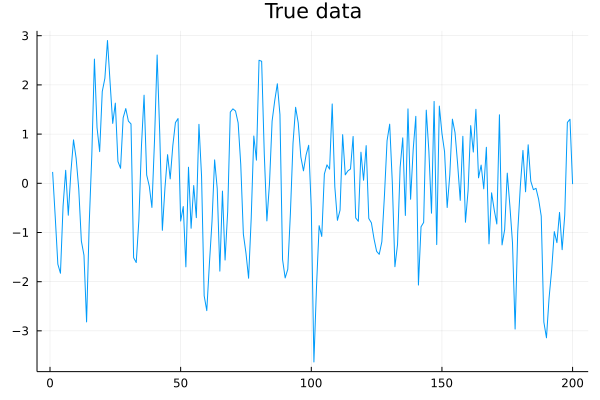
\includegraphics[scale=0.4]{x_plot.png}
    \end{center}
\end{sol}
\begin{problem}{4}
\end{problem}
\begin{sol}
    We begin by considering the vector for the case where $m_2$ uses only the mean and variance. We expect that there will be a significant problem here, since the mean is not informative about the parameters of the data generating process. This means our coefficients will likely be under-identified: we only have one real informative moment, meaning that we cannot independently pin down $\rho$ and $\sigma^2$ based on the variance alone. To see why, we note that we could have $\frac{\sigma^2}{1-\rho^2} = 1$ either if $\sigma^2$ is really high and $\rho$ is really low, or if $\sigma^2 $ is really low and $\rho$ is really high. This means that when we are searching for a minimum, there are basically two opposite directions we can go. As such, we are likely to run into issues of consistency here.
    \begin{enumerate}[label=\alph*) ]
        \item The plot of the objective function with $W = I$ is included below:
        \begin{center}
            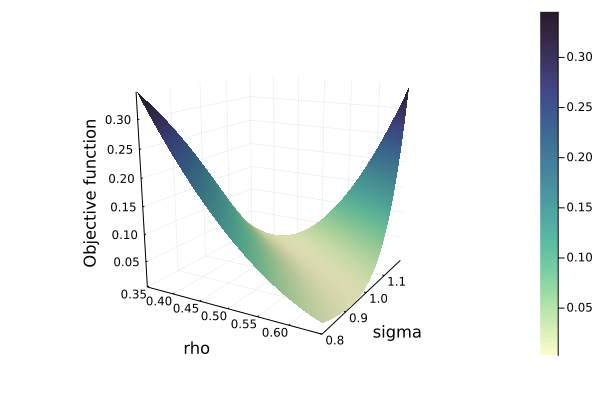
\includegraphics[scale=0.4]{jthplot_1_init.png}
        \end{center}
        Importantly, we note that the objective function is flat on the diagonal where $\sigma^2$ decreases as $\rho$ increases. This is precisely related to the above argument that the same value of $\frac{\sigma^2}{1-\rho^2}$ can be generated by high $\sigma^2$ and low $\rho$ or low $\sigma^2$ and high $\rho$. We expect that our optimization algorithm will have trouble with this valley.

        Finding the minimum of the objective function, we estimate that
        \[\hat{\beta}_{TH}^1 = \begin{bmatrix} -1.0158 \\ 0.0005\end{bmatrix}\]
        This is very far off from the true, which is not immediately disconcerting given that we know we have insufficient moments to identify this model.
        \item We now construct an estimate of $W^*$ and use it to find $\hat{b}_{TH}^2$. We can do so by computing $\hat{W}_TH = \hat{S}_TH^{-1}$. We find that
        \[\hat{W}_{TH} = \begin{bmatrix}2.8775 & 0.0036\\ 0.0036& 0.022\end{bmatrix}\]
        We now use this to find the second stage objective function, which we minimize to find $\hat{b}_TH^2$. The new objective function with $\hat{W}_{TH}$ is included below:
        \begin{center}
            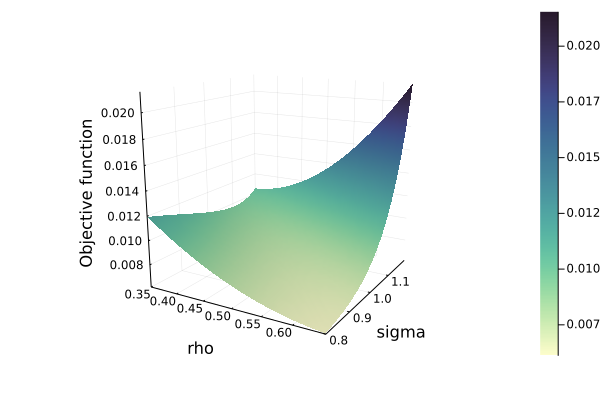
\includegraphics[scale=0.4]{jthplot_1_2nd.png}
        \end{center}
        Minimizing the new objective function induced by $\hat{W}_TH$, we obtain that
        \[\hat{b}_{TH} = \begin{bmatrix}-1.0231 \\0.0001\end{bmatrix}\]
        Again, this is$\ldots$not great. But we expect bad performance given that we only have one informative moment.
        \item We numerically compute $\nabla_b g_T(\hat{b}_TH^2)$ and include our results below:
        \[\nabla_b g_T(\hat{b}_{TH}^2) \approx \begin{bmatrix}-0.1773 &8.0654\\ 420.044 & -19550.8225\end{bmatrix}\]
        The variance-covariance matrix of $\hat{b}_TH^2$ is equal to $\frac{1}{T}[\nabla_b g_T(\hat{b}_{TH}^2) \hat{W}_{TH} \nabla_b g_T(\hat{b}_{TH}^2)]^{-1}$, which we compute below:
        \[\begin{bmatrix}105.3784 & 2.264\\ 2.264& 0.0486 \end{bmatrix}\]
        Finally, taking the square root of the diagonal of this matrix, we find the standard errors for $\hat{\rho}_TH^2$ and $\hat{\sigma}_TH^2$, respectively:
        \[se(\hat{b}_{TH}^2) = \begin{bmatrix} 10.2654\\ 0.2205\end{bmatrix}\]
        Not surprisingly, the standard error of $\rho$ is just massive. 
        \item Finally, we compute the value of the $J$ statistic given by
        \[J = T \frac{H}{1 + H}\times J_{TH}(\hat{b}_{TH}^2) = 0.1244\]
        Under the null hypothesis, the $J$ statistic should follow a $\chi^2$ distribution. We note that $P(\chi^2 > 0.1244) = 0.2757$, meaning the $p$ value of the $J$ test is 0.2754. 
    \end{enumerate}
\end{sol}
\begin{problem}{5}
\end{problem}
\begin{sol}
    We now consider the just-identified case where $m_2$ uses the mean and autocovariance. We do not expect the same problem, as we now have multiple moments which will hopefully allow us to pin down $\rho$ and $\sigma^2$ separately.
    \begin{enumerate}[label=\alph*) ]
        \item The plot of the objective function with $W = I$ is included below:
        \begin{center}
            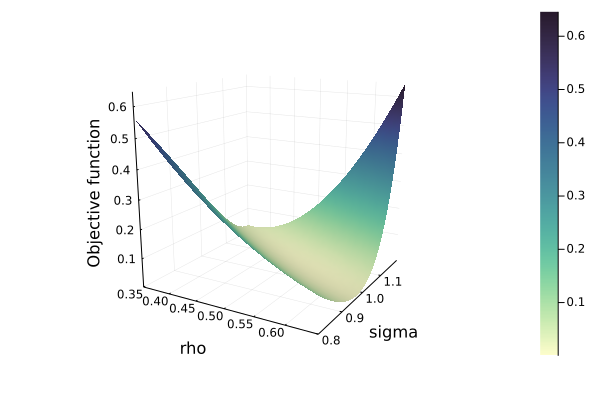
\includegraphics[scale=0.4]{jthplot_2_init.png}
        \end{center}
        
        Finding the minimum of the objective function, we estimate that
        \[\hat{\beta}_{TH}^1 = \begin{bmatrix} 0.5271 \\ 1.0835\end{bmatrix}\]
        This is far closer to the true parameters than the previous estimate, which is reassuring. 
        \item We now construct an estimate of $W^*$ and use it to find $\hat{b}_{TH}^2$. We can do so by computing $\hat{W}_TH = \hat{S}_TH^{-1}$. We find that
        \[\hat{W}_{TH} = \begin{bmatrix} 0.49 & -0.4858\\ -0.4858 & 0.6319\end{bmatrix}\]
        We now use this to find the second stage objective function, which we minimize to find $\hat{b}_TH^2$. The new objective function with $\hat{W}_{TH}$ is included below:
        \begin{center}
            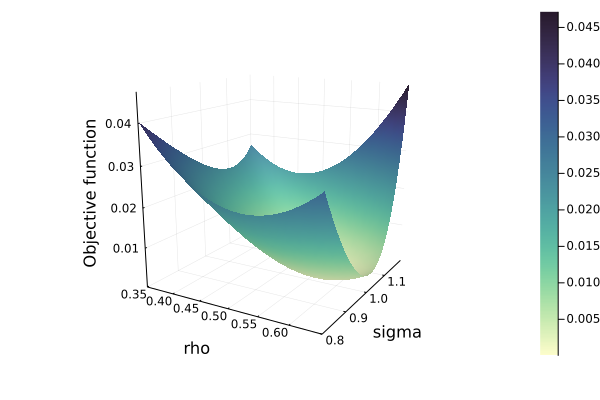
\includegraphics[scale=0.4]{jthplot_2_2nd.png}
        \end{center}
        Minimizing the new objective function induced by $\hat{W}_TH$, we obtain that
        \[\hat{b}_{TH} = \begin{bmatrix}0.5271\\1.0834\end{bmatrix}\]
        We can see that our parameter estimates barely changed at all from the first stage.
        \item We numerically compute $\nabla_b g_T(\hat{b}_TH^2)$ and include our results below:
        \[\nabla_b g_T(\hat{b}_{TH}^2) \approx \begin{bmatrix}-2.194  &-1.3807\\ -2.658& -0.7155\end{bmatrix}\]
        The variance-covariance matrix of $\hat{b}_TH^2$ is equal to $\frac{1}{T}[\nabla_b g_T(\hat{b}_{TH}^2) \hat{W}_{TH} \nabla_b g_T(\hat{b}_{TH}^2)]^{-1}$, which we compute below:
        \[\begin{bmatrix} 0.0046 & -0.0022\\ -0.0022 & 0.0178\end{bmatrix}\]
        Finally, taking the square root of the diagonal of this matrix, we find the standard errors for $\hat{\rho}_TH^2$ and $\hat{\sigma}_TH^2$, respectively:
        \[se(\hat{b}_{TH}^2) = \begin{bmatrix} 0.0677\\ 0.1335\end{bmatrix}\]
        Reassuringly, these standard errors are far lower than previously! The benefits of using the right moments are clearly large.
        \item Finally, we compute the value of the $J$ statistic given by
        \[J = T \frac{H}{1 + H}\times J_{TH}(\hat{b}_{TH}^2) = 4 \times 10^{-7}\]
        Under the null hypothesis, the $J$ statistic should follow a $\chi^2$ distribution. We note that $P(\chi^2 > 4\times 10^{-7}) \approx 0.0005$, meaning the $p$ value of the $J$ test is very close to zero. This is consistent with what it should be.
    \end{enumerate}
\end{sol}
\begin{problem}{6}
\end{problem}
\begin{sol}
    We now consider the case where we use the mean, variance, and first order autocovariance to construct $m_3$. We don't expect there to be a problem, since we have more than enough moments to identify the model parameters. However, we may be a bit worried about including extraneous moments.
    \begin{enumerate}[label=\alph*) ]
        \item The plot of the objective function with $W = I$ is included below:
        \begin{center}
            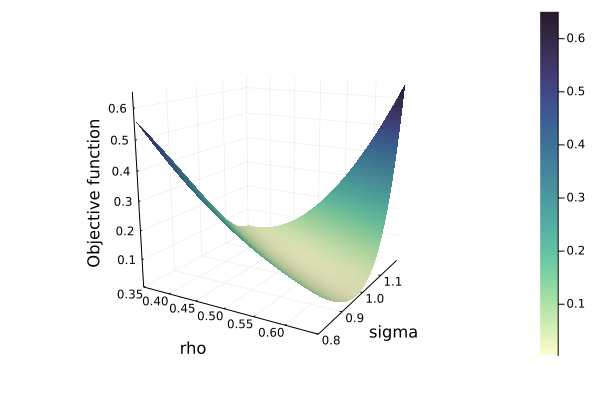
\includegraphics[scale=0.4]{jthplot_3_init.png}
        \end{center}
        
        Finding the minimum of the objective function, we estimate that
        \[\hat{\beta}_{TH}^1 = \begin{bmatrix} 0.5258 \\1.0857\end{bmatrix}\]
        This is very close to our estimate for the just-identified case when we used the variance and autocovariance.
        \item We now construct an estimate of $W^*$ and use it to find $\hat{b}_{TH}^2$. We can do so by computing $\hat{W}_TH = \hat{S}_TH^{-1}$. We find that
        \[\hat{W}_{TH} = \begin{bmatrix} 0.315 &0.0084&0.0138\\ 0.0084 &0.4885& -0.4835\\ 0.0138 &-0.4835& 0.6308\end{bmatrix}\]
        We now use this to find the second stage objective function, which we minimize to find $\hat{b}_TH^2$. The new objective function with $\hat{W}_{TH}$ is included below:
        \begin{center}
            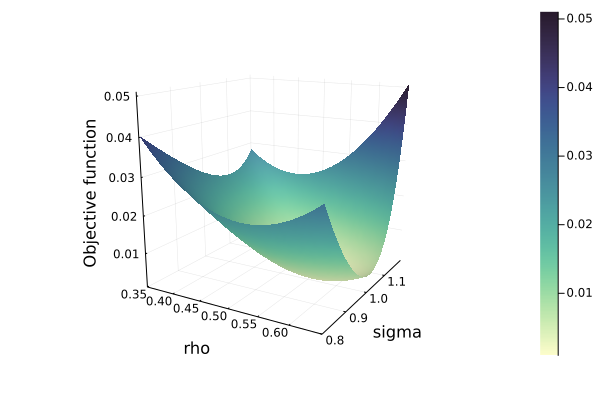
\includegraphics[scale=0.4]{jthplot_3_2nd.png}
        \end{center}
        Minimizing the new objective function induced by $\hat{W}_TH$, we obtain that
        \[\hat{b}_{TH} = \begin{bmatrix}0.5239\\ 1.0802\end{bmatrix}\]
        Like last time, the parameter estimates don't change too much, although they changed more than in the just-identified case. Notably, the estimates for $\rho$ and $\sigma^2$ moved farther closer to their true values.
        \item We numerically compute $\nabla_b g_T(\hat{b}_TH^2)$ and include our results below:
        \[\nabla_b g_T(\hat{b}_{TH}^2) \approx \begin{bmatrix}-0.078 &-0.0168\\ -2.1534& -1.3742\\ -2.6186 &-0.7077\end{bmatrix}\]
        The variance-covariance matrix of $\hat{b}_TH^2$ is equal to $\frac{1}{T}[\nabla_b g_T(\hat{b}_{TH}^2) \hat{W}_{TH} \nabla_b g_T(\hat{b}_{TH}^2)]^{-1}$, which we compute below:
        \[\begin{bmatrix} 0.0046 &-0.0022\\ -0.0022 &0.0178\end{bmatrix}\]
        Finally, taking the square root of the diagonal of this matrix, we find the standard errors for $\hat{\rho}_TH^2$ and $\hat{\sigma}_TH^2$, respectively:
        \[se(\hat{b}_{TH}^2) = \begin{bmatrix} 0.068\\ 0.1332\end{bmatrix}\]
        These standard errors are very similar to the standard errors of the just-identified case using the variance and autocovariance.
        \item Finally, we compute the value of the $J$ statistic given by
        \[J = T \frac{H}{1 + H}\times J_{TH}(\hat{b}_{TH}^2) = 0.1595\]
        Under the null hypothesis, the $J$ statistic should follow a $\chi^2$ distribution. We note that $P(\chi^2 > 0.1595) \approx 0.3104$, meaning the $p$ value of the $J$ test is approximately $0.3104$. 
        \item Finally, we do $B=1000$ bootstrap replications of the above procedure and find the mean of the bootstrap parameter estimates:
        \[E[\hat{\rho}_{TH}^1] = 0.4932\]
        \[E[\hat{\rho}_{TH}^2] = 0.4936\]
        \[E[\hat{\sigma^2}_{TH}^1] = 1.0061\]
        \[E[\hat{\sigma^2}_{TH}^2] = 1.0040\]
        We also plot the histograms of the bootstrap distributions for each estimator below:
        \begin{center}
            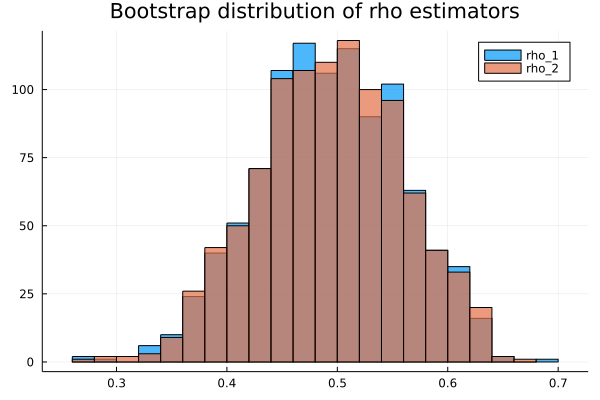
\includegraphics[scale=0.5]{rho_bootstrap.png}
        \end{center}
        \begin{center}
            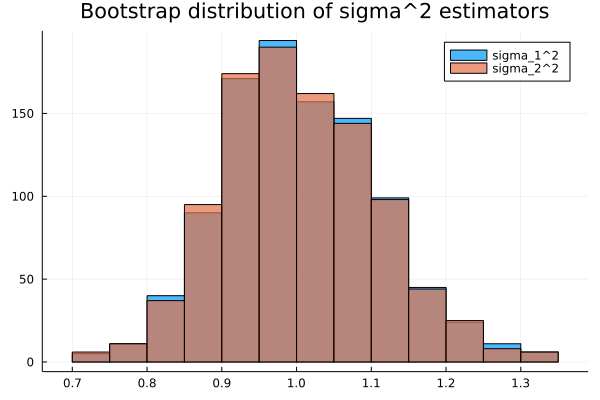
\includegraphics[scale=0.5]{sigma_bootstrap.png}
        \end{center}
    \end{enumerate}
\end{sol}

\end{document}